\chapter{Regular Surfaces}\label{chap:surfaces}

% ==================== Section 2-1: Introduction ====================
\section{Introduction}\label{sec:surfaces-intro}

\textbf{From curves to surfaces.} 在第一章中，我们研究了 $\mathbb{R}^3$ 中的曲线理论。通过引入曲率和挠率，我们学会了如何用精确的数学语言描述曲线的"弯曲程度"。自然的问题是：能否将类似的理论推广到二维甚至更高维的对象？

这一想法引导我们进入曲面理论。与曲线不同的是，曲面是"二维"的——它们在每一点附近都像一个平面。正如曲线需要正则性（避免尖点）以便定义切线，曲面也需要某种正则性条件以保证切平面（tangent plane）的存在。

\textbf{The main theme.} 本章研究 $\mathbb{R}^3$ 中曲面的微分几何。我们将看到，曲面为二元函数的微积分提供了天然的研究框架。事实上，曲面论正是高斯（Gauss）和黎曼（Riemann）开创现代微分几何的起点。

\textbf{Organization of this chapter.} 本章内容安排如下。2-2 节引入正则曲面（regular surface）的基本概念，这是全书的基础；2-3 节讨论曲面上的可微函数；2-4 节引入第一基本形式（first fundamental form），用于处理曲面上的度量问题（弧长、面积等）。

\textbf{Why surfaces?} 曲面之所以重要，有多重原因。首先，现实世界中的许多物体（地球表面、电影屏幕、弯曲的镜片）都是曲面而非曲线。其次，曲面理论是理解弯曲空间（曲面的内蕴几何）的起点——高斯称之为"非凡的定理"（Theorema Egregium）：曲面的曲率可以仅用曲面自身的度量来定义，而不依赖于它如何嵌入 $\mathbb{R}^3$。这一发现深刻地影响了物理学中广义相对论的发展。

\begin{figure}[H]
\centering
\begin{minipage}{0.45\textwidth}
\centering
\subfloat[Figure 2-1. 正则曲面的参数化]{\label{fig:fig2-1}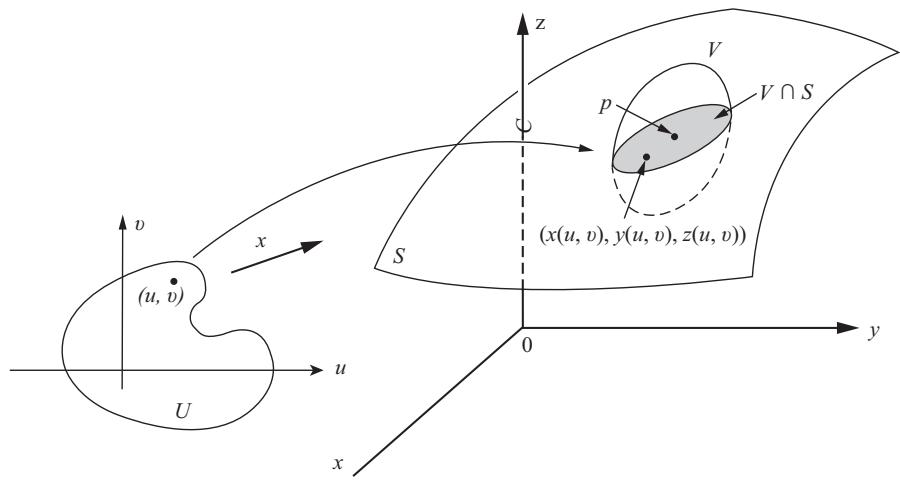
\includegraphics[width=\textwidth]{../../../PDFs/differential-geometry/transcript/Do Carmo - Differential Geometry of Curves and Surfaces/hybrid_ocr/images/9182b715913ef41534ac27f5769d97aea20063b58fd9d15ca1b4ef11da858ff1.jpg}}
\end{minipage}
\hfill
\begin{minipage}{0.45\textwidth}
\centering
\subfloat[Figure 2-2. 坐标曲线与切向量]{\label{fig:fig2-2}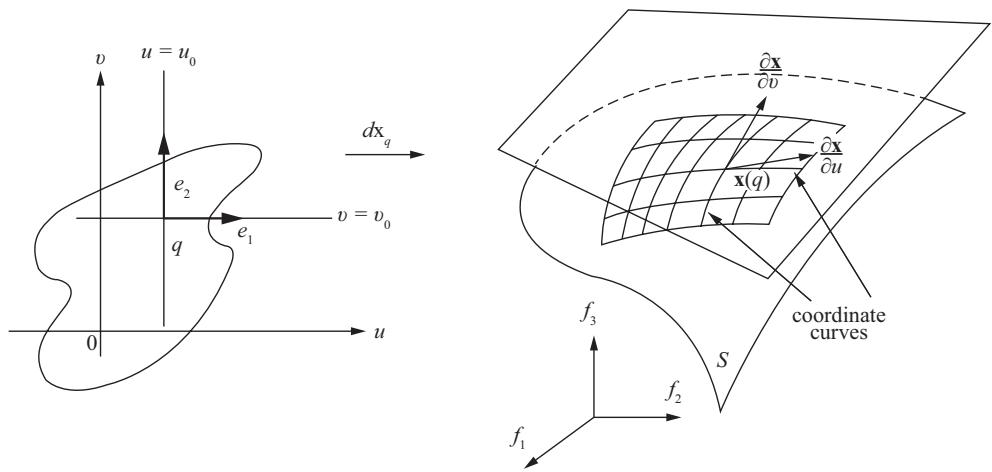
\includegraphics[width=\textwidth]{../../../PDFs/differential-geometry/transcript/Do Carmo - Differential Geometry of Curves and Surfaces/hybrid_ocr/images/14fe34e73ea93e0d8038fe79aff12b40bf5ece89780624d7e112f6143d6d1a63.jpg}}
\end{minipage}
\end{figure}

% ==================== Section 2-2: Regular Surfaces ====================
\section{Regular Surfaces; Inverse Images of Regular Values}\label{sec:regular-surfaces}

\textbf{Defining a surface.} 如何精确地定义"曲面"？直观上，曲面是 $\mathbb{R}^3$ 中的一块"二维"片状结构，它没有尖点、没有自交，并且在每一点处都有良好的切平面。

与曲线的定义方式不同（曲线是参数化映射），我们定义曲面为 $\mathbb{R}^3$ 的一个子集。原因是：曲面作为"面"，应该是独立于参数化而存在的几何对象。

\begin{Definition}[正则曲面]\label{def:regular-surface}
设 $S \subset \mathbb{R}^3$。如果对每一点 $p \in S$，存在 $\mathbb{R}^3$ 中的邻域 $V$ 和映射
\[
\mathbf{x}: U \subset \mathbb{R}^2 \to V \cap S,
\]
其中 $U$ 是 $\mathbb{R}^2$ 中的开集，使得（见 \cref{fig:fig2-1}，教材 Figure 2-1）：
\begin{enumerate}
\item $\mathbf{x}$ 是可微的。这意味着如果写
\[
\mathbf{x}(u,v) = (x(u,v), y(u,v), z(u,v)),\quad (u,v) \in U,
\]
则函数 $x(u,v), y(u,v), z(u,v)$ 在 $U$ 上有所有阶的连续偏导数。

\item $\mathbf{x}$ 是同胚。即 $\mathbf{x}$ 连续且有连续的逆映射 $\mathbf{x}^{-1}: V \cap S \to U$。

\item（正则条件）对每个 $q \in U$，微分 $d\mathbf{x}_q: \mathbb{R}^2 \to \mathbb{R}^3$ 是单射。
\end{enumerate}
则称 $S$ 为\textbf{\underline{正则曲面}}（regular surface）。
\end{Definition}

映射 $\mathbf{x}$ 称为 $p$ 邻域的\textbf{\underline{参数化}}（parametrization）或\textbf{\underline{局部坐标}}（system of (local) coordinates）。

\textbf{The regularity condition.} 条件 3 至关重要。回顾：$d\mathbf{x}_q$ 在标准基下的矩阵为
\[
d\mathbf{x}_q = \begin{pmatrix}
\frac{\partial x}{\partial u} & \frac{\partial x}{\partial v} \\
\frac{\partial y}{\partial u} & \frac{\partial y}{\partial v} \\
\frac{\partial z}{\partial u} & \frac{\partial z}{\partial v}
\end{pmatrix}.
\]

条件 3 要求这两列向量线性无关——即向量 $\partial\mathbf{x}/\partial u$ 和 $\partial\mathbf{x}/\partial v$ 不平行。几何上，这意味着在 $p$ 点处存在良好定义的切平面。

\begin{Remark}
让我们逐一解释这三个条件的几何意义：
\begin{itemize}
\item 条件 1（可微性）保证曲面是"光滑"的，能够进行微分运算；
\item 条件 2（单射性）防止自交——如果曲面与自身相交，就无法谈论"在 $p$ 点的切平面"；
\item 条件 3（正则条件）保证每点都有良好定义的切平面。
\end{itemize}
这三个条件共同确保了曲面上的微分几何是有意义的。
\end{Remark}

\begin{figure}[H]
\centering
\begin{minipage}{0.45\textwidth}
\centering
\subfloat[Figure 2-3 (a). 自交情形 — 不能定义唯一切平面]{\label{fig:fig2-3a}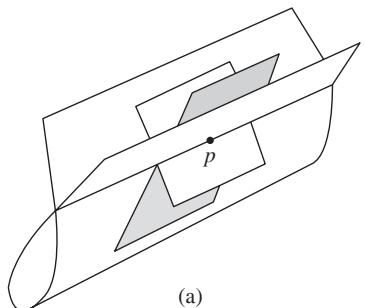
\includegraphics[width=\textwidth]{../../../PDFs/differential-geometry/transcript/Do Carmo - Differential Geometry of Curves and Surfaces/hybrid_ocr/images/982f74acb26628a48d71a466dae574fef45a04dbcf320fcb5714a526f10cd8ed.jpg}}
\end{minipage}
\hfill
\begin{minipage}{0.45\textwidth}
\centering
\subfloat[Figure 2-3 (b). 正则曲面 — 每点有良好定义的切平面]{\label{fig:fig2-3b}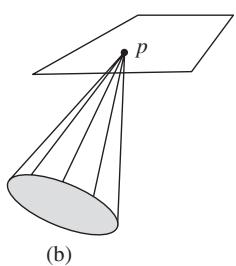
\includegraphics[width=\textwidth]{../../../PDFs/differential-geometry/transcript/Do Carmo - Differential Geometry of Curves and Surfaces/hybrid_ocr/images/0020313622314d0c333e47f99980b4ef05e0c8ac53e5c0910d29805904e23797.jpg}}
\end{minipage}
\end{figure}

\begin{Example}[单位球面]\label{ex:sphere}
单位球面
\[
S^2 = \{(x,y,z) \in \mathbb{R}^3; x^2 + y^2 + z^2 = 1\}
\]
是正则曲面。

我们用六个参数化来覆盖整个球面。例如，定义 $\mathbf{x}_1: U \subset \mathbb{R}^2 \to \mathbb{R}^3$ 为
\[
\mathbf{x}_1(x,y) = (x, y, +\sqrt{1-(x^2+y^2)}),\quad (x,y) \in U,
\]
其中 $U = \{(x,y) \in \mathbb{R}^2; x^2 + y^2 < 1\}$。

验证三个条件：
\begin{enumerate}
\item $\mathbf{x}_1$ 是可微的（因为 $x^2+y^2<1$ 时根号内为正）；
\item $\mathbf{x}_1$ 是单射，逆映射是投影 $\pi(x,y,z) = (x,y)$；
\item 雅可比行列式 $\frac{\partial(x,y)}{\partial(x,y)} \equiv 1 \neq 0$。
\end{enumerate}

类似地定义 $\mathbf{x}_2$（下半球）、$\mathbf{x}_3, \mathbf{x}_4$（$xz$ 平面投影）、$\mathbf{x}_5, \mathbf{x}_6$（$yz$ 平面投影），这六个参数化共同覆盖整个球面（见 \cref{fig:fig2-4}，教材 Figure 2-4）。
\end{Example}

\begin{figure}[H]
\centering
\begin{minipage}{0.7\textwidth}
\centering
\subfloat[Figure 2-4. 球面的六个参数化邻域]{\label{fig:fig2-4}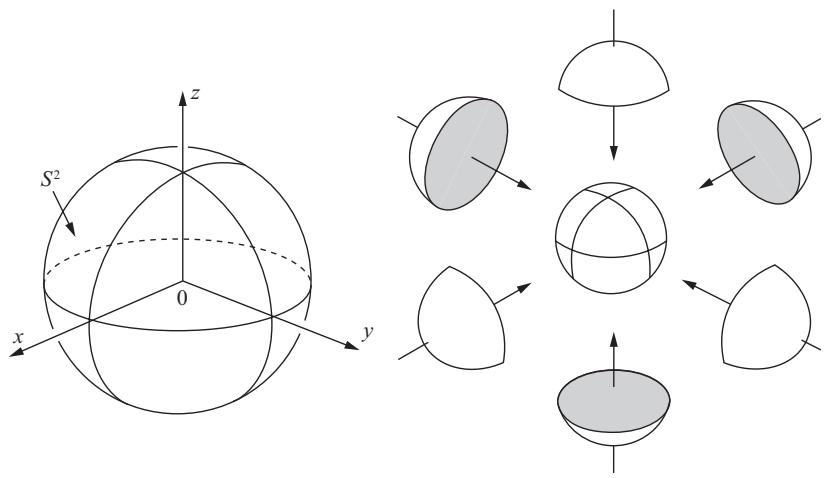
\includegraphics[width=\textwidth]{../../../PDFs/differential-geometry/transcript/Do Carmo - Differential Geometry of Curves and Surfaces/hybrid_ocr/images/b0f439063c9a3837b427e9f827366c854cdb5ae59b8c0eb305664cba91fa43a6.jpg}}
\end{minipage}
\end{figure}

\textbf{Geographical coordinates.} 对于大多数应用，更方便的是使用球面坐标。设
\[
V = \{(\theta, \varphi); 0 < \theta < \pi,\; 0 < \varphi < 2\pi\},
\]
定义 $\mathbf{x}: V \to \mathbb{R}^3$ 为（见 \cref{fig:fig2-5}，教材 Figure 2-5）
\[
\mathbf{x}(\theta, \varphi) = (\sin\theta\cos\varphi,\; \sin\theta\sin\varphi,\; \cos\theta).
\]
这里 $\theta$ 是余纬度（colatitude），$\varphi$ 是经度（longitude）。
\begin{figure}[H]
\centering
\begin{minipage}{0.5\textwidth}
\centering
\subfloat[Figure 2-5. 球面坐标 $\theta$ 和 $\varphi$]{\label{fig:fig2-5}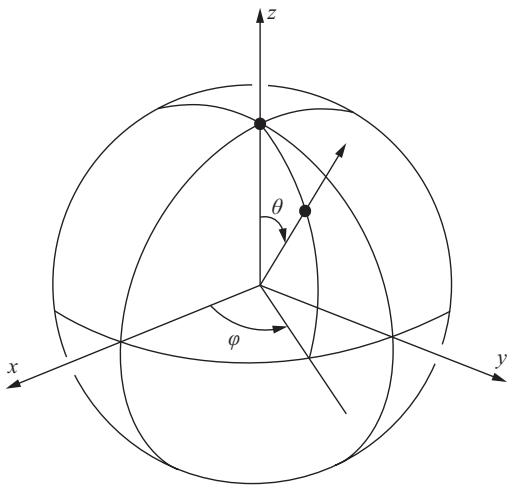
\includegraphics[width=\textwidth]{../../../PDFs/differential-geometry/transcript/Do Carmo - Differential Geometry of Curves and Surfaces/hybrid_ocr/images/29b4cf1487ab401a9c3132cb791f96ac850e3b26e7a0a1b77ea146f3315d284b.jpg}}
\end{minipage}
\end{figure}

\begin{Proposition}[垂直投影判断法]\label{prop:graph-criterion}
设 $S \subset \mathbb{R}^3$。如果对每一点 $p \in S$，存在 $p$ 的邻域 $V$ 使得 $V \cap S$ 是以下三种形式之一：
\[
z = f(x,y),\quad y = g(x,z),\quad x = h(y,z),
\]
其中 $f,g,h$ 是可微函数，则 $S$ 是正则曲面。
\end{Proposition}

\textbf{Why is this useful?} 这个命题告诉我们：判断一个集合是否是曲面，只需检查它局部是否是某个可微函数的图像。这比直接验证定义中的三个条件要容易得多。

\begin{Example}[旋转面]\label{ex:surface-of-revolution}
设 $C$ 是 $xz$ 平面中的一条光滑曲线，绕 $z$ 轴旋转得到的曲面是正则曲面（如果 $C$ 不与 $z$ 轴相交）。例如，环面（torus）就是由椭圆绕 $z$ 轴旋转而成的。

旋转面的参数化可以写成
\[
\mathbf{x}(u,v) = ((r\cos u + a)\cos v,\; (r\cos u + a)\sin v,\; r\sin u),
\]
其中 $0 < u, v < 2\pi$（见 \cref{fig:fig2-9}，教材 Figure 2-9）。
\end{Example}

\begin{figure}[H]
\centering
\begin{minipage}{0.6\textwidth}
\centering
\subfloat[Figure 2-9. 环面 (torus)]{\label{fig:fig2-9}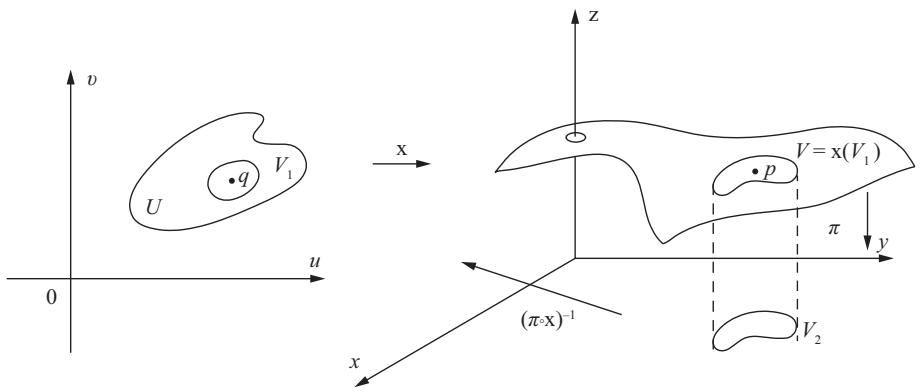
\includegraphics[width=\textwidth]{../../../PDFs/differential-geometry/transcript/Do Carmo - Differential Geometry of Curves and Surfaces/hybrid_ocr/images/abf059759e9ec36e5b4e3fdbafd96373e1127c14a7e600e0f029e4745e090361.jpg}}
\end{minipage}
\end{figure}

\begin{Example}[锥面不是正则曲面]\label{ex:cone-not-regular}
单叶锥面
\[
C = \{(x,y,z) \in \mathbb{R}^3; z = +\sqrt{x^2+y^2}\}
\]
\textbf{不是}正则曲面。关键在于顶点 $(0,0,0)$ 处——任何包含该点的邻域都与锥面相交，而在该点处无法定义良好的切平面（锥面在顶点处有一个"尖"）。

这个例子说明了定义中条件 3 的必要性：如果仅仅去掉顶点，修改后的曲面将是正则的。
\end{Example}

\subsection*{2-2 节练习}

\begin{exercise}{2-2, 1 — do Carmo, Exercise 2-2, 1}
Show that the cylinder $\{(x,y,z)\in \mathbb{R}^3;x^2 +y^2 = 1\}$ is a regular surface, and find parametrizations whose coordinate neighborhoods cover it.
\end{exercise}

\begin{solution}
\textbf{直观理解}：柱面是由圆周沿垂直方向平移得到的。我们可以利用隐函数定理（正则值命题）来证明其正则性，或者直接构造参数化。

\textbf{证明}：
设 $f(x,y,z) = x^2 + y^2$。柱面是集合 $f^{-1}(1)$。
计算梯度：$\nabla f = (2x, 2y, 0)$。
在柱面上，$x^2 + y^2 = 1$，故 $(x,y) \neq (0,0)$，从而 $\nabla f \neq (0,0,0)$。
根据正则值命题，$1$ 是 $f$ 的正则值，故 $f^{-1}(1)$ 是正则曲面。

\textbf{参数化}：
取 $\mathbf{x}_1(u,v) = (\cos u, \sin u, v)$，$u \in (0, 2\pi)$，$v \in \mathbb{R}$。
取 $\mathbf{x}_2(u,v) = (\cos u, \sin u, v)$，$u \in (-\pi, \pi)$，$v \in \mathbb{R}$。
这两个局部坐标邻域的并集覆盖了整个柱面。$\square$
\end{solution}

\begin{exercise}{2-2, 2 — do Carmo, Exercise 2-2, 2}
Is the set $\{(x,y,z)\in \mathbb{R}^3;z = 0$ and $x^{2} + y^{2}\leq 1\}$ a regular surface? Is the set $\{(x,y,z)\in \mathbb{R}^3;z = 0$, and $x^{2} + y^{2} < 1\}$ a regular surface?
\end{exercise}

\begin{solution}
\textbf{解答}：
1. 闭圆盘 $S_1 = \{(x,y,z); z=0, x^2+y^2 \leq 1\}$ \textbf{不是}正则曲面。
原因：对于边界点 $p = (1,0,0) \in S_1$，任何包含 $p$ 的邻域 $V \cap S_1$ 在 $p$ 点附近只有一侧有定义，它不 homeomorphic 到 $\mathbb{R}^2$ 中的一个开集。

2. 开圆盘 $S_2 = \{(x,y,z); z=0, x^2+y^2 < 1\}$ \textbf{是}正则曲面。
原因：它是平面 $z=0$（一个正则曲面）的一个开子集，或者可以直接视为函数 $z = 0$ 在开集 $x^2+y^2 < 1$ 上的图像。
\end{solution}

\begin{exercise}{2-2, 3 — do Carmo, Exercise 2-2, 3}
Show that the two-sheeted cone, with its vertex at the origin, that is, the set $\{(x,y,z)\in \mathbb{R}^3;x^2 +y^2 -z^2 = 0\}$, is not a regular surface.
\end{exercise}

\begin{solution}
\textbf{证明}：
考虑原点 $O = (0,0,0)$。在 $O$ 的任何邻域内，锥面由两部分构成，它们在顶点处相交。
如果锥面是正则曲面，则在 $O$ 点应存在切平面。但由方程 $f(x,y,z) = x^2+y^2-z^2 = 0$ 确定的曲面，其梯度 $\nabla f = (2x, 2y, -2z)$ 在原点处为零向量。
更形式化地，原点的任何邻域与锥面的交集在去掉原点后有两个连通分支，这与 $\mathbb{R}^2$ 中开盘去掉一点后仍连通的拓扑性质矛盾。因此它不是正则曲面。$\square$
\end{solution}

\begin{exercise}{2-2, 4 — do Carmo, Exercise 2-2, 4}
Let $f(x, y, z) = z^2$. Prove that $0$ is not a regular value of $f$ and yet that $f^{-1}(0)$ is a regular surface.
\end{exercise}

\begin{solution}
\textbf{证明}：
1. $\nabla f = (0, 0, 2z)$。在 $f(x,y,z) = 0$（即 $z=0$）处，$\nabla f = (0,0,0)$。故 $0$ 不是 $f$ 的正则值。
2. 然而，$f^{-1}(0) = \{(x,y,z); z^2 = 0\} = \{(x,y,z); z = 0\}$。
这恰好是 $xy$ 平面，它是正则曲面（可视为函数 $z = 0$ 的图像）。
这说明"正则值"是判定正则曲面的充分而非必要条件。$\square$
\end{solution}

\begin{exercise}{2-2, 5* — do Carmo, Exercise 2-2, 5}
Let $P = \{(x, y, z) \in \mathbb{R}^3; x = y\}$ (a plane) and let $\mathbf{x}: U \subset \mathbb{R}^2 \to \mathbb{R}^3$ be given by
\[
\mathbf{x}(u, v) = (u + v, u + v, uv),
\]
where $U = \{(u,v)\in \mathbb{R}^2;u > v\}$. Clearly, $\mathbf{x}(U)\subset P$. Is $\mathbf{x}$ a parametrization of $P$?
\end{exercise}

\begin{solution}
\textbf{直观理解}：我们需要验证 $\mathbf{x}$ 是否满足正则曲面定义的三个条件。

\textbf{解答}：
1. 可微性：显然。
2. 正则性：计算偏导向量
\[
\mathbf{x}_u = (1, 1, v), \quad \mathbf{x}_v = (1, 1, u).
\]
其外积为 $\mathbf{x}_u \wedge \mathbf{x}_v = (u-v, v-u, 0)$。
因为在 $U$ 上 $u > v$，故 $u-v \neq 0$，外积永不为零。正则性满足。
3. 同胚性：$\mathbf{x}$ 必须是单射且逆连续。
由 $x = u+v$, $z = uv$ 知 $u, v$ 是方程 $t^2 - xt + z = 0$ 的两个根。
由于 $u > v$，这两个根被唯一确定。判别式 $D = x^2 - 4z = (u-v)^2 > 0$。
这表明 $\mathbf{x}(U)$ 是平面 $P$ 中满足 $x^2 > 4z$ 的部分。这是一个开集，且映射是单射。
由于它只是覆盖了 $P$ 的一部分，它不是整个 $P$ 的参数化，但是它是其像 $\mathbf{x}(U) \subset P$ 的一个合法参数化。$\square$
\end{solution}

\begin{exercise}{2-2, 6 — do Carmo, Exercise 2-2, 6}
Give another proof of Prop. 1 by applying Prop. 2 to $h(x, y, z) = f(x, y) - z$.
\end{exercise}

\begin{solution}
\textbf{证明}：
设曲面是函数 $z = f(x,y)$ 的图像。构造辅助函数 $h(x,y,z) = f(x,y) - z$。
则曲面可表示为 $h^{-1}(0)$。
计算梯度：$\nabla h = (f_x, f_y, -1)$。
由于第三个分量恒为 $-1$，梯度 $\nabla h$ 在任何点都不为零向量。
根据命题 2（正则值命题），$0$ 是 $h$ 的正则值，故 $h^{-1}(0)$ 是正则曲面。$\square$
\end{solution}

\begin{exercise}{2-2, 7 — do Carmo, Exercise 2-2, 7}
Let $f(x, y, z) = (x + y + z - 1)^2$.
\begin{enumerate}
\item[a.] Locate the critical points and critical values of $f$.
\item[b.] For what values of $c$ is the set $f(x, y, z) = c$ a regular surface?
\item[c.] Answer the questions of parts a and b for the function $f(x, y, z) = xyz^2$.
\end{enumerate}
\end{exercise}

\begin{solution}
\textbf{解答}：
\textbf{a.} $\nabla f = 2(x+y+z-1)(1, 1, 1)$。
临界点：$x+y+z-1 = 0$（整个平面）。
临界值：$f(\text{临界点}) = 0^2 = 0$。

\textbf{b.} 当 $c \neq 0$ 且 $c > 0$ 时（因为 $f \geq 0$），$c$ 是正则值。
但需注意：对于 $c > 0$，$f^{-1}(c)$ 由两个平行平面 $x+y+z-1 = \pm\sqrt{c}$ 组成，它们是正则曲面。
当 $c = 0$ 时，$f^{-1}(0)$ 是平面 $x+y+z-1 = 0$，也是正则曲面（即便 $0$ 不是正则值）。
当 $c < 0$ 时，集合为空。

\textbf{c.} 对于 $f = xyz^2$：
$\nabla f = (yz^2, xz^2, 2xyz)$。
临界点：
1. $z=0$（整个 $xy$ 平面）；
2. $x=0, y=0$（$z$ 轴）。
临界值：$f(x,y,0) = 0$，$f(0,0,z) = 0$。故唯一临界值是 $0$。
当 $c \neq 0$ 时，$f^{-1}(c)$ 是正则曲面。
\end{solution}

\begin{exercise}{2-2, 8* — do Carmo, Exercise 2-2, 8}
Let $\mathbf{x}(u, v)$ be as in Def. 1. Verify that $d\mathbf{x}_q: \mathbb{R}^2 \to \mathbb{R}^3$ is one-to-one if and only if
\[
\frac{\partial \mathbf{x}}{\partial u} \wedge \frac{\partial \mathbf{x}}{\partial v} \neq 0.
\]
\end{exercise}

\begin{solution}
\textbf{证明}：
线性映射 $d\mathbf{x}_q$ 是单射当且仅当其雅可比矩阵的秩为 2。
雅可比矩阵的两列恰好是向量 $\mathbf{x}_u$ 和 $\mathbf{x}_v$。
在 $\mathbb{R}^3$ 中，两个向量线性无关当且仅当它们不共线。
而 $\mathbf{x}_u \wedge \mathbf{x}_v = 0$ 当且仅当 $\mathbf{x}_u$ 与 $\mathbf{x}_v$ 线性相关。
故 $d\mathbf{x}_q$ 是单射当且仅当 $\mathbf{x}_u \wedge \mathbf{x}_v \neq 0$。$\square$
\end{solution}

\begin{exercise}{2-2, 9 — do Carmo, Exercise 2-2, 9}
Let $V$ be an open set in the $xy$ plane. Show that the set
\[
\{(x, y, z) \in \mathbb{R}^3; z = 0 \text{ and } (x, y) \in V\}
\]
is a regular surface.
\end{exercise}

\begin{solution}
\textbf{证明}：
该集合是平面 $z = 0$ 的一个开子集。
取参数化 $\mathbf{x}(u,v) = (u,v,0)$，其中 $(u,v) \in V$。
1. $\mathbf{x}$ 显然可微；
2. $\mathbf{x}$ 是恒等映射，显然是同胚；
3. $\mathbf{x}_u \wedge \mathbf{x}_v = (1,0,0) \wedge (0,1,0) = (0,0,1) \neq 0$。
因此它是正则曲面。$\square$
\end{solution}

\begin{exercise}{2-2, 10* — do Carmo, Exercise 2-2, 10}
Let $C$ be a figure "8" in the $xy$ plane and let $S$ be the cylindrical surface over $C$ (见 \cref{fig:fig2-11}，教材 Figure 2-11); that is,
\[
S = \{(x, y, z) \in \mathbb{R}^3; (x, y) \in C \}.
\]
Is the set $S$ a regular surface?
\end{exercise}

\begin{solution}
\textbf{解答}：
\textbf{不是}。
原因在于 "8" 字曲线的交点 $p$。在 $S$ 中，通过该交点的任何邻域都包含两条相交的竖直带状区域。
这类似于练习 3 中的锥面顶点，该点附近的局部拓扑不是一个开盘（它是一个"十字形"的局部结构）。
正式地说，在该交点处无法定义唯一的切平面，且该点任何邻域去掉后会分成四个分支，不 homeomorphic 到 $\mathbb{R}^2$。
\end{solution}

\begin{figure}[H]
\centering
\begin{minipage}{0.5\textwidth}
\centering
\subfloat[Figure 2-11. 8字曲线生成的柱面]{\label{fig:fig2-11}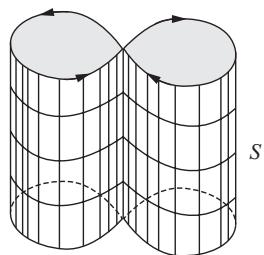
\includegraphics[width=\textwidth]{../../../PDFs/differential-geometry/transcript/Do Carmo - Differential Geometry of Curves and Surfaces/hybrid_ocr/images/989523d17639b5f31f0ed0e2d4d9077a348942766a19d1143dd29cf290eae71d.jpg}}
\end{minipage}
\end{figure}

% ==================== Section 2-3: Change of Parameters ====================
\section{Change of Parameters; Differentiable Functions on Surfaces}\label{sec:change-of-params}

在上一节中，我们看到正则曲面可以用不同的参数化来描述。例如，球面可以用地理坐标 $(\theta, \varphi)$，也可以用平面垂直投影的六个局部坐标卡来描述。重要的是，\textbf{由曲面本身决定的几何量}（如切平面）不应该依赖于参数化的选择。

\textbf{Why do we need different parametrizations?} 一个参数化 $\mathbf{x}: U \to S$ 只能覆盖曲面的一部分。例如，球面的地理坐标参数化在两极处失效（雅可比为零）。因此，我们需要多个参数化来覆盖整个曲面。

不同参数化之间的关系由\textbf{坐标变换}（change of parameters）描述。如果 $\mathbf{x}: U \to S$ 和 $\tilde{\mathbf{x}}: \tilde{U} \to S$ 是两个有重叠区域的参数化，则在重叠区域上有坐标变换
\[
\Phi = \mathbf{x}^{-1} \circ \tilde{\mathbf{x}}: \tilde{U}' \to U,
\]
其中 $\tilde{U}' \subset \tilde{U}$ 是重叠区域在 $\tilde{\mathbf{x}}$ 下的像。

\begin{Proposition}[坐标变换是可微的]\label{prop:change-of-params}
设 $\mathbf{x}: U \to S$ 和 $\tilde{\mathbf{x}}: \tilde{U} \to S$ 是正则曲面 $S$ 的两个参数化，假设 $\mathbf{x}^{-1}(\mathbf{x}(U) \cap \tilde{\mathbf{x}}(\tilde{U})) \subset U$。则坐标变换 $\Phi = \mathbf{x}^{-1} \circ \tilde{\mathbf{x}}$ 是可微的。
\end{Proposition}

\textbf{This is important.} 这个命题告诉我们：无论我们用哪个参数化来计算，曲面上的可微函数的概念是良好定义的。一个函数 $f: S \to \mathbb{R}$ 在点 $p$ 处可微，意味着它在某个（从而任何）参数化下是可微的。

\begin{Definition}[曲面上的可微函数]\label{def:differentiable-function-on-surface}
设 $f: S \to \mathbb{R}$ 是定义在正则曲面 $S$ 上的函数。如果对每一点 $p \in S$，存在参数化 $\mathbf{x}: U \to S$ 使得 $p \in \mathbf{x}(U)$，且合成函数
\[
f \circ \mathbf{x}: U \subset \mathbb{R}^2 \to \mathbb{R}
\]
在 $q = \mathbf{x}^{-1}(p)$ 处是可微的，则称 $f$ 在 $p$ 处\textbf{\underline{可微}}（differentiable）。
\end{Definition}

类似地，可以定义可微映射 $F: S_1 \to S_2$。

\begin{Remark}
这个定义的关键在于：它不依赖于参数化的选择。如果一个函数在一个参数化下是可微的，它在所有参数化下都是可微的。
\end{Remark}

\begin{Example}[高度函数]\label{ex:height-function}
设 $S$ 是单位球面，定义高度函数 $f: S \to \mathbb{R}$ 为 $f(x,y,z) = z$。在地理坐标下，$f(\mathbf{x}(\theta,\varphi)) = \cos\theta$，这是可微的。因此 $f$ 是 $S$ 上的可微函数。
\end{Example}

\begin{Definition}[可微曲线]\label{def:differentiable-curve-on-surface}
曲面 $S$ 上的\textbf{可微曲线}是可微映射 $\alpha: I \subset \mathbb{R} \to S$，其中 $I$ 是区间。
\end{Definition}

\textbf{Connection with Chapter 1.} 注意到如果 $\alpha: I \to S$ 是曲面 $S$ 上的可微曲线，则作为 $\mathbb{R}^3$ 中的曲线，$\alpha$ 也是可微的（因为包含映射 $i: S \hookrightarrow \mathbb{R}^3$ 是嵌入）。

\subsection*{2-3 节练习}

\begin{exercise}{2-3, 1 — do Carmo, Exercise 2-3, 1}
Let $S^2 = \{(x,y,z) \in \mathbb{R}^3; x^2 + y^2 + z^2 = 1\}$ be the unit sphere and let $f: S^2 \to \mathbb{R}$ be given by $f(x,y,z) = z$. Show that $f$ is differentiable.
\end{exercise}

\begin{solution}
\textbf{证明}：
根据可微函数的定义，我们只需在覆盖球面的参数化下检查 $f \circ \mathbf{x}$ 的可微性。
1. 在地理坐标下，$\mathbf{x}(\theta, \varphi) = (\sin\theta\cos\varphi, \sin\theta\sin\varphi, \cos\theta)$。
则 $f(\mathbf{x}(\theta, \varphi)) = \cos\theta$。这是一个关于 $(\theta, \varphi)$ 的 $C^\infty$ 函数。
2. 在投影参数化下，如 $\mathbf{x}(x,y) = (x, y, \sqrt{1-x^2-y^2})$。
则 $f(\mathbf{x}(x,y)) = \sqrt{1-x^2-y^2}$。在开盘 $x^2+y^2 < 1$ 内，这也是 $C^\infty$ 的。
由于 $f$ 在局部参数化下均可微，故 $f$ 是 $S^2$ 上的可微函数。$\square$
\end{solution}

\begin{exercise}{2-3, 2 — do Carmo, Exercise 2-3, 2}
Let $S \subset \mathbb{R}^3$ be a regular surface and let $p \in S$. Show that there exists a neighborhood $V$ of $p$ in $S$ such that the projection onto the tangent plane at $p$ maps $V$ diffeomorphically onto an open set of $\mathbb{R}^2$.
\end{exercise}

\begin{solution}
\textbf{证明}：
设 $T_pS$ 为切空间。我们可以选择一个旋转和平移，使得 $p$ 位于原点且 $T_pS$ 为 $xy$ 平面。
此时，单位法向量 $N(p) = (0,0,1)$。
考虑投影 $\pi: S \to \mathbb{R}^2$，$\pi(x,y,z) = (x,y)$。
其微分 $d\pi_p: T_pS \to \mathbb{R}^2$ 是恒等映射（因为 $T_pS$ 本身就是 $xy$ 平面）。
由于 $d\pi_p$ 是同构，根据反函数定理，存在 $p$ 的邻域 $V \subset S$，使得 $\pi|_V$ 是微分同胚。$\square$
\end{solution}

\begin{exercise}{2-3, 3* — do Carmo, Exercise 2-3, 3}
Let $\mathbf{x}: U \to S$ be a parametrization of a regular surface $S$. Show that $\mathbf{x}^{-1}: \mathbf{x}(U) \to U$ is continuous. (This shows that condition 2 in the definition of a regular surface can be replaced by: $\mathbf{x}$ is a homeomorphism onto its image.)
\end{exercise}

\begin{solution}
\textbf{证明}：
根据正则曲面的定义，$\mathbf{x}$ 是可微映射且其微分 $d\mathbf{x}_q$ 在每一点都是单射。
根据反函数定理的推广形式，$\mathbf{x}$ 在局部是开映射。
这意味着对 $U$ 中的任何开集 $W$，$\mathbf{x}(W)$ 是 $\mathbf{x}(U)$ 中的开集。
由拓扑学知识，一个连续的双射如果将开集映射为开集，则其逆映射必连续。
因此 $\mathbf{x}^{-1}$ 是连续的，即 $\mathbf{x}$ 是同胚。$\square$
\end{solution}

\begin{exercise}{2-3, 4 — do Carmo, Exercise 2-3, 4}
Let $F: S_1 \to S_2$ be a differentiable map between regular surfaces. Show that the set of critical points of $F$ is closed in $S_1$.
\end{exercise}

\begin{solution}
\textbf{证明}：
临界点是满足 $\text{rank}(dF_p) < 2$ 的点 $p$。
在局部参数化下，$dF_p$ 由 $2 \times 2$ 的雅可比矩阵 $J$ 表示。
$\text{rank}(J) < 2$ 等价于 $\det(J) = 0$。
由于 $F$ 是可微的，$dF_p$ 的分量是连续函数，故其行列式 $\det(J)$ 也是 $p$ 的连续函数。
临界点集是连续函数 $\det(J)$ 的零点集，故在每个坐标邻域内是闭的。
因此，整个临界点集在 $S_1$ 中是闭集。$\square$
\end{solution}

\begin{exercise}{2-3, 5 — do Carmo, Exercise 2-3, 5}
Show that the map $F: S^2 \to S^2$ given by $F(x,y,z) = (-x,y,z)$ (a rotation by $\pi$ around the $y$-axis) is differentiable. Find the matrix of $dF_p$ in an appropriate basis.
\end{exercise}

\begin{solution}
\textbf{解答}：
1. 可微性：$F$ 是 $\mathbb{R}^3$ 线性变换限制在 $S^2$ 上。由于 $\mathbb{R}^3$ 中的线性变换是 $C^\infty$ 的，且 $S^2$ 是子流形，故 $F$ 是可微的。
2. 微分矩阵：在 $p$ 点，取 $T_pS^2$ 的基。
由于 $F$ 是线性映射，$dF_p$ 实际上就是该线性映射本身在切空间上的限制。
如果在 $\mathbb{R}^3$ 下，$F$ 的矩阵为 $A = \begin{pmatrix} -1 & 0 & 0 \\ 0 & 1 & 0 \\ 0 & 0 & 1 \end{pmatrix}$。
对于 $v \in T_pS^2$，有 $dF_p(v) = Av$。
若取合适基（如 $p$ 点切平面上的正交基），则矩阵形式取决于 $p$ 的位置。$\square$
\end{solution}

% ==================== Section 2-4: The Differential of a Map ====================
\section{The Differential of a Map; Tangent Plane}\label{sec:differential-tangent-plane}

... (content omitted) ...

\subsection*{2-4 节练习}

\begin{exercise}{2-4, 1 — do Carmo, Exercise 2-4, 1}
Let $S \subset \mathbb{R}^3$ be a regular surface and let $p \in S$. Show that $T_pS$ depends only on the set $S$, not on the parametrization used in its definition.
\end{exercise}

\begin{solution}
\textbf{证明}：
切空间 $T_pS$ 定义为通过 $p$ 点的所有曲面内可微曲线在 $p$ 点切向量的集合。
这个定义只涉及到集合 $S$ 和其上的可微结构（即哪些曲线被视为可微）。
虽然我们常用参数化 $\mathbf{x}_u, \mathbf{x}_v$ 来构造基，但命题 1 证明了不同参数化生成的向量空间是相同的。
因此 $T_pS$ 是曲面的内在几何对象。$\square$
\end{solution}

\begin{exercise}{2-4, 2* — do Carmo, Exercise 2-4, 2}
Let $F: S_1 \to S_2$ be a differentiable map between regular surfaces. Show that $dF_p: T_pS_1 \to T_{F(p)}S_2$ is a linear map.
\end{exercise}

\begin{solution}
\textbf{证明}：
在局部坐标下，设 $\alpha(t)$ 是 $S_1$ 上的曲线，$v = \alpha'(0)$。
$dF_p(v) = (F \circ \alpha)'(0)$。
根据多元微积分的链式法则，在参数化 $\mathbf{x}$ 和 $\mathbf{y}$ 下，这对应于雅可比矩阵乘以向量 $v$ 的坐标。
矩阵相乘是线性变换，因此 $dF_p$ 是线性的。$\square$
\end{solution}

\begin{exercise}{2-4, 3 — do Carmo, Exercise 2-4, 3}
Let $F: S \to \mathbb{R}$ be a differentiable function on a regular surface $S$. Show that the set of critical points of $F$ is closed in $S$.
\end{exercise}

\begin{solution}
\textbf{证明}：
临界点是 $dF_p = 0$ 的点。在局部参数化下，$dF_p$ 是由偏导数 $(F_u, F_v)$ 构成的向量。
由于 $F$ 是可微的，$F_u$ 和 $F_v$ 是连续函数。
临界点集是方程 $F_u(p) = 0$ 和 $F_v(p) = 0$ 的解集。
这是连续函数零点的交集，故是闭集。$\square$
\end{solution}

\begin{exercise}{2-4, 4 — do Carmo, Exercise 2-4, 4}
Let $S^2 = \{(x,y,z); x^2+y^2+z^2 = 1\}$ and let $F: S^2 \to \mathbb{R}$ be given by $F(x,y,z) = z$. Find all critical points of $F$ and compute $dF_p$ at each critical point.
\end{exercise}

\begin{solution}
\textbf{解答}：
1. 临界点：$F$ 是高度函数。在球面 $S^2$ 上，$F$ 在北极 $(0,0,1)$ 取得最大值，在南极 $(0,0,-1)$ 取得最小值。
在极值点处，导数必为零。
事实上，在任何其他点，高度方向的投影在切平面上都不为零。
故临界点为 $N = (0,0,1)$ 和 $S = (0,0,-1)$。
2. 微分：在临界点处，$dF_p$ 是零映射。$\square$
\end{solution}

\begin{exercise}{2-4, 5* — do Carmo, Exercise 2-4, 5}
Let $F: S_1 \to S_2$ be a differentiable map between regular surfaces. Show that if $F$ is a diffeomorphism (i.e., $F$ is invertible and both $F$ and $F^{-1}$ are differentiable), then $dF_p: T_pS_1 \to T_{F(p)}S_2$ is an isomorphism for all $p \in S_1$.
\end{exercise}

\begin{solution}
\textbf{证明}：
根据链式法则，$F^{-1} \circ F = \text{id}_{S_1}$ 意味着
\[
d(F^{-1})_{F(p)} \circ dF_p = d(\text{id})_p = \text{Id}_{T_pS_1}.
\]
同理，$dF_p \circ d(F^{-1})_{F(p)} = \text{Id}_{T_{F(p)}S_2}$。
这表明 $dF_p$ 有逆映射 $d(F^{-1})_{F(p)}$。
由于 $dF_p$ 及其逆映射都是线性映射，故 $dF_p$ 是切空间之间的同构。$\square$
\end{solution}

\begin{exercise}{2-4, 6 — do Carmo, Exercise 2-4, 6}
Let $S \subset \mathbb{R}^3$ be a regular surface and let $p \in S$. Show that the tangent plane $T_pS$ can be characterized as the set of vectors $v \in \mathbb{R}^3$ such that $v \cdot N(p) = 0$, where $N(p)$ is a normal vector to $S$ at $p$.
\end{exercise}

\begin{solution}
\textbf{证明}：
根据定义，切空间 $T_pS$ 是由 $\mathbf{x}_u$ 和 $\mathbf{x}_v$ 张成的二维空间。
而单位法向量 $N(p)$ 定义为 $\frac{\mathbf{x}_u \wedge \mathbf{x}_v}{|\mathbf{x}_u \wedge \mathbf{x}_v|}$，显然垂直于 $\mathbf{x}_u$ 和 $\mathbf{x}_v$。
因此，任何切向量 $v \in T_pS$ 必与 $N(p)$ 正交。
反之，由于 $\mathbb{R}^3$ 中与 $N(p)$ 正交的向量构成一个二维空间，而 $T_pS$ 也是一个与之重合的二维空间，故二者等价。$\square$
\end{solution}

% ==================== Section 2-5: The First Fundamental Form ====================
\section{The First Fundamental Form}\label{sec:first-fundamental-form}

在定义了切平面之后，我们现在可以讨论曲面上的度量几何。回想第一章中曲线的弧长公式：对于单位速度曲线 $\alpha(s)$，弧长就是 $s$。对于曲面，我们需要类似的概念来测量曲线上两点之间的弧长，以及曲面的面积。

\textbf{From curves to arc length on surfaces.} 设 $\alpha: [a,b] \to S$ 是曲面 $S$ 上的可微曲线。则 $\alpha$ 作为 $\mathbb{R}^3$ 中的曲线，其弧长为
\[
L(\alpha) = \int_a^b \|\alpha'(t)\| \, dt.
\]
但 $\|\alpha'(t)\|^2 = \alpha'(t) \cdot \alpha'(t)$，这是一个依赖于 $\alpha'(t)$ 的二次型。我们将会看到，这个二次型恰好是曲面的第一基本形式。

\begin{Definition}[第一基本形式]\label{def:first-fundamental-form}
设 $p \in S$，$v \in T_pS$。定义\textbf{\underline{第一基本形式}}（first fundamental form）$I_p: T_pS \times T_pS \to \mathbb{R}$ 为
\[
I_p(v, w) = v \cdot w.
\]
即切空间上的标准内积。
\end{Definition}

第一基本形式衡量的是切向量之间的角度和长度关系。由于它源自 $\mathbb{R}^3$ 的内积，它实际上就是限制在切平面上的内积。

\begin{Proposition}[弧长公式]\label{prop:arc-length-first-form}
设 $\alpha: [a,b] \to S$ 是曲面 $S$ 上的可微曲线。则其弧长为
\[
L(\alpha) = \int_a^b \sqrt{I_{\alpha(t)}(\alpha'(t), \alpha'(t))} \, dt = \int_a^b \|\alpha'(t)\| \, dt.
\]
\end{Proposition}

在参数化曲面 $\mathbf{x}(u,v)$ 下，切向量 $\alpha'(t) = \mathbf{x}_u u'(t) + \mathbf{x}_v v'(t)$，所以
\[
\|\alpha'(t)\|^2 = E(u'(t))^2 + 2F u'(t) v'(t) + G(v'(t))^2,
\]
其中
\[
E = \mathbf{x}_u \cdot \mathbf{x}_u,\quad F = \mathbf{x}_u \cdot \mathbf{x}_v,\quad G = \mathbf{x}_v \cdot \mathbf{x}_v.
\]

\begin{Definition}[Gauss 系数]\label{def:gauss-coefficients}
量 $E, F, G$ 称为曲面的\textbf{\underline{Gauss 系数}}（Gauss coefficients）。它们完全决定了曲面的第一基本形式。
\end{Definition}

\begin{Example}[平面]\label{ex:plane-first-form}
设 $S$ 是 $xy$ 平面，参数化为 $\mathbf{x}(u,v) = (u,v,0)$。则
\[
E = 1,\quad F = 0,\quad G = 1.
\]
第一基本形式为 $I = du^2 + dv^2$。这正是平面几何中的弧长公式。
\end{Example}

\begin{Example}[球面]\label{ex:sphere-first-form}
在地理坐标下，单位球面的参数化为
\[
\mathbf{x}(\theta,\varphi) = (\sin\theta\cos\varphi,\; \sin\theta\sin\varphi,\; \cos\theta).
\]
计算得
\[
E = 1,\quad F = 0,\quad G = \sin^2\theta.
\]
第一基本形式为 $I = d\theta^2 + \sin^2\theta\, d\varphi^2$。

特别地，在纬度 $\theta$ 处，一度的经线弧长为 $d\theta$，一度的纬线弧长为 $\sin\theta\, d\varphi$。
\end{Example}

\textbf{Why does this matter?} 第一基本形式是曲面的"内在度量"——它只依赖于曲面本身，而不依赖于曲面如何嵌入 $\mathbb{R}^3$。高斯著名的 Theorema Egregium 指出：曲面的曲率（ Gauss 曲率）可以完全用 $E, F, G$ 及其导数来表示。这意味着曲率是曲面的内在性质，不随曲面在空间中的弯曲而改变。

\begin{Proposition}[曲面的面积]\label{prop:surface-area}
设 $R \subset U$ 是参数化 $\mathbf{x}: U \to S$ 的定义域中的一个区域。则 $\mathbf{x}(R)$ 在曲面 $S$ 上的面积为
\[
A(\mathbf{x}(R)) = \iint_R \|\mathbf{x}_u \times \mathbf{x}_v\| \, du\, dv = \iint_R \sqrt{EG - F^2}\, du\, dv.
\]
\end{Proposition}

这里 $\|\mathbf{x}_u \times \mathbf{x}_v\| = \sqrt{EG - F^2}$ 是两个切向量张成的平行四边形的面积。

\begin{Example}[球冠的面积]\label{ex:sphere-cap-area}
考虑单位球面在 $z \geq c$ 部分（$0 < c < 1$）。使用地理坐标，这部分对应 $0 \leq \theta \leq \theta_0$，其中 $\cos\theta_0 = c$。

面积
\[
A = \int_0^{2\pi} \int_0^{\theta_0} \sin\theta\, d\theta\, d\varphi = 2\pi(1 - c).
\]
特别地，当 $c = 0$（半球面）时，面积为 $2\pi$。
\end{Example}

\subsection*{2-5 节练习}

\begin{exercise}{2-5, 1 — do Carmo, Exercise 2-5, 1}
Let $S \subset \mathbb{R}^3$ be a regular surface and let $p \in S$. Show that the first fundamental form $I_p$ is a positive definite bilinear form on $T_pS$.
\end{exercise}

\begin{exercise}{2-5, 2 — do Carmo, Exercise 2-5, 2}
Let $S$ be the cylinder $x^2 + y^2 = 1$. Compute the first fundamental form in the parametrization $\mathbf{x}(u,v) = (\cos u, \sin u, v)$.
\end{exercise}

\begin{exercise}{2-5, 3 — do Carmo, Exercise 2-5, 3}
Let $S$ be the surface of revolution obtained by rotating the curve $z = f(x)$, $x > 0$, around the $z$-axis. Find the first fundamental form in the natural parametrization.
\end{exercise}

\begin{exercise}{2-5, 4* — do Carmo, Exercise 2-5, 4}
Show that the area $A$ of a region $R$ on a surface $S$ is given by
\[
A = \iint_R d\sigma,
\]
where $d\sigma = \sqrt{EG - F^2}\, du\, dv$ is the element of area.
\end{exercise}

\begin{exercise}{2-5, 5 — do Carmo, Exercise 2-5, 5}
Let $T$ be the torus with parameters as in Example 6 of Sec. 2-2. Compute the area of $T$.
\end{exercise}

\begin{exercise}{2-5, 6 — do Carmo, Exercise 2-5, 6}
Let $S$ be a regular surface and let $p \in S$. Show that the angle $\theta$ between two curves $\alpha, \beta$ on $S$ intersecting at $p$ satisfies
\[
\cos\theta = \frac{I_p(\alpha'(0), \beta'(0))}{\|\alpha'(0)\| \|\beta'(0)\|}.
\]
\end{exercise}

% ==================== Section 2-6: Orientation ====================
\section{Orientation on Surfaces}\label{sec:orientation}

\textbf{Why orientation?} 对于曲线，我们可以通过切向量 $\alpha'(t)$ 的符号来判断运动方向。对于曲面，我们需要类似的概念来区分"两侧"——比如一张纸有正面和反面。

在 $\mathbb{R}^3$ 中，每个正则曲面在每一点处都有两个单位法向量，它们恰好相反。选择其中一个连续变化的法向量场，就是给曲面一个定向（orientation）。

\begin{Definition}[可定向曲面]\label{def:orientable}
正则曲面 $S$ 称为\textbf{\underline{可定向的}}（orientable），如果存在连续的可微映射 $N: S \to \mathbb{R}^3$ 使得对每一点 $p \in S$，$N(p)$ 是 $S$ 在 $p$ 处的单位法向量。
\end{Definition}

\begin{Example}[球面是可定向的]\label{ex:sphere-orientable}
单位球面 $S^2$ 是可定向的。单位法向量场可以取为 $N(x,y,z) = (x,y,z)$。这是连续可微的。
\end{Example}

\begin{Example}[Möbius 带是不可定向的]\label{ex:mobius-not-orientable}
Möbius 带是\textbf{不可定向}的经典例子。如果你沿着 Möbius 带走一圈，法向量的方向会翻转。这与 Möbius 带只有一个面有关——你不需要翻过边缘就能到达"另一面"。
\end{Example}

\textbf{Practical criterion.} 判断曲面是否可定向，可以检查是否存在整体定义的连续法向量场。对于大多数常见的曲面（如球面、环面、平面），这是成立的。

\begin{Proposition}[可定向的等价条件]\label{prop:orientable-equivalent}
正则曲面 $S$ 是可定向的，当且仅当存在 $S$ 的一个参数化覆盖，使得所有参数化的坐标变换的雅可比行列式都为正。
\end{Proposition}

这个命题的几何意义是：可定向意味着我们可以在整个曲面上一致地选择"左手系"或"右手系"的局部坐标。

\begin{Remark}
曲面的定向在后续章节中很重要。例如，在学习曲面的面积分和 Stokes 定理时，需要选择一致的定向。
\end{Remark}

\subsection*{2-6 节练习}

\begin{exercise}{2-6, 1 — do Carmo, Exercise 2-6, 1}
Show that the cylinder $x^2 + y^2 = 1$ is orientable.
\end{exercise}

\begin{exercise}{2-6, 2* — do Carmo, Exercise 2-6, 2}
Show that the Möbius band is not orientable.
\end{exercise}

\begin{exercise}{2-6, 3 — do Carmo, Exercise 2-6, 3}
Let $S$ be a regular surface covered by two parametrizations $\mathbf{x}_1: U_1 \to S$ and $\mathbf{x}_2: U_2 \to S$. Show that if the overlap $\mathbf{x}_1(U_1) \cap \mathbf{x}_2(U_2)$ is connected, then the orientability of $S$ is equivalent to the Jacobian of the coordinate change $\mathbf{x}_2^{-1} \circ \mathbf{x}_1$ being positive on $U_1 \cap \mathbf{x}_1^{-1}(\mathbf{x}_2(U_2))$.
\end{exercise}

% ==================== Section 2-7: Geometry of the Gauss Map ====================
\section{Geometry of the Gauss Map}\label{sec:gauss-map}

\textbf{The Gauss map.} 在定义了切平面之后，我们现在可以讨论曲面的"弯曲"程度。正如曲线的曲率描述其弯曲程度，曲面的 Gauss 映射描述了曲面如何"远离"其切平面。

\begin{Definition}[Gauss 映射]\label{def:gauss-map}
设 $S \subset \mathbb{R}^3$ 是可定向的正则曲面，$N: S \to S^2$ 是单位法向量场。定义\textbf{\underline{Gauss 映射}}（Gauss map）为
\[
N: S \to S^2,
\]
它将 $S$ 上每一点映射到单位球面上对应的法向量。
\end{Definition}

Gauss 映射的几何直觉是：将曲面每一点的法向量"压缩"到单位球面上。如果曲面在某点附近平坦，法向量变化缓慢，Gauss 映射的像就小；如果曲面弯曲剧烈，法向量变化剧烈，Gauss 映射的像就大。

\textbf{This is remarkable.} 高斯发现：Gauss 映射的微分 $dN_p$ 的行列式（取绝对值）恰好是曲面的曲率。这意味着曲率可以通过纯内在的量（法向量场的变化）来计算——这就是著名的 Theorema Egregium。

\begin{Definition}[Gauss 曲率]\label{def:gauss-curvature}
设 $p \in S$，$K(p) = \det(dN_p)$。则 $K(p)$ 称为 $S$ 在 $p$ 处的\textbf{\underline{Gauss 曲率}}（Gauss curvature）。
\end{Definition}

\begin{Example}[平面的曲率为零]\label{ex:plane-curvature}
设 $S$ 是 $xy$ 平面。单位法向量场为常数 $N(x,y,z) = (0,0,1)$。因此 $dN_p = 0$ 对所有 $p$ 成立，故 $K \equiv 0$。这符合直觉——平面完全不弯曲。
\end{Example}

\begin{Example}[球面的曲率为正]\label{ex:sphere-curvature}
单位球面的单位法向量场为 $N(x,y,z) = (x,y,z)$。在地理坐标下，直接计算可得 $K \equiv 1$。这意味着球面在每一点都"正向弯曲"。
\end{Example}

\begin{Example}[马鞍面的曲率为负]\label{ex:saddle-curvature}
曲面 $z = x^2 - y^2$（双曲抛物面，或称"马鞍面"）在原点处的 Gauss 曲率为负。这意味着在该点处，曲面在一个方向向上弯曲，在垂直方向向下弯曲。
\end{Example}

\begin{Proposition}[曲率的符号]\label{prop:curvature-sign}
设 $p \in S$，$K(p)$ 是 Gauss 曲率。
\begin{itemize}
\item 如果 $K(p) > 0$，则曲面在 $p$ 点附近是"椭圆"的（如球面）；
\item 如果 $K(p) = 0$，则曲面在 $p$ 点是抛物或平直的（如平面、柱面）；
\item 如果 $K(p) < 0$，则曲面在 $p$ 点是双曲的（如马鞍面）。
\end{itemize}
\end{Proposition}

\begin{Remark}
Gauss 曲率的符号告诉我们曲面在局部是向哪一侧弯曲：
\begin{itemize}
\item $K > 0$：曲面全部位于切平面的一侧
\item $K = 0$：曲面与切平面有多重接触（如柱面的直母线方向）
\item $K < 0$：曲面穿过切平面（如马鞍面）
\end{itemize}
\end{Remark}

\begin{Definition}[平均曲率]\label{def:mean-curvature}
设 $k_1, k_2$ 为主曲率（principal curvatures），即 $dN_p$ 的特征值。则\textbf{\underline{平均曲率}}（mean curvature）为
\[
H = \frac{k_1 + k_2}{2}.
\]
\end{Definition}

平均曲率在极小曲面理论中起重要作用——平均曲率为零的曲面是极小曲面（minimal surface）。

\subsection*{2-7 节练习}

\begin{exercise}{2-7, 1 — do Carmo, Exercise 2-7, 1}
Show that the Gauss curvature $K$ of a regular surface $S$ satisfies
\[
K = \frac{\det(dN_p)}{\det(d\mathbf{x}_p)},
\]
where $d\mathbf{x}_p$ is the differential of a parametrization at $p$.
\end{exercise}

\begin{exercise}{2-7, 2 — do Carmo, Exercise 2-7, 2}
Compute the Gauss curvature of the cylinder $x^2 + y^2 = 1$.
\end{exercise}

\begin{exercise}{2-7, 3* — do Carmo, Exercise 2-7, 3}
Show that the Theorema Egregium holds: the Gauss curvature $K$ of a surface can be expressed in terms of the first fundamental form coefficients $E, F, G$ and their derivatives.
\end{exercise}

\begin{exercise}{2-7, 4 — do Carmo, Exercise 2-7, 4}
Let $S$ be a surface of revolution. Show that the Gauss curvature at a point depends only on the distance of the point from the axis of revolution.
\end{exercise}

\begin{exercise}{2-7, 5 — do Carmo, Exercise 2-7, 5}
Show that if $K > 0$ everywhere on a connected surface $S$, then no geodesic on $S$ can have a conjugate point.
\end{exercise}

% ==================== Section 2-8: Parallel Transport; Geodesics ====================
\section{Parallel Transport; Geodesics}\label{sec:geodesics}

\textbf{From straight lines to geodesics.} 在平面上，直线是两点之间的最短路径。在曲面上，直线的类比是\textbf{测地线}（geodesic）——它是局部最短的曲线。

测地线的概念源于一个简单的问题：在曲面上，什么是"直线"的类比？答案是：曲率为零的曲线。但这需要一个更深入的概念——协变导数（covariant derivative）和\textbf{平行移动}（parallel transport）。

\begin{Definition}[协变导数]\label{def:covariant-derivative}
设 $S$ 是正则曲面，$\alpha: I \to S$ 是可微曲线，$V(t)$ 是 $\alpha$ 上的切向量场。$\alpha$ 上的\textbf{协变导数} $\frac{DV}{dt}$ 定义为 $V'(t)$ 在切平面 $T_{\alpha(t)}S$ 上的正交投影。
\end{Definition}

协变导数告诉我们：沿曲线移动向量时，其变化中有多少是"垂直于曲面"的。剩余的"切向"部分就是在曲面上的真实变化。

\begin{Definition}[平行移动]\label{def:parallel-transport}
设 $\alpha: [a,b] \to S$ 是曲面 $S$ 上的可微曲线。沿 $\alpha$ 的\textbf{平行移动}是将切向量从 $T_{\alpha(a)}S$ 传输到 $T_{\alpha(b)}S$ 的过程，使得被移动的向量 $V(t)$ 满足协变导数 $\frac{DV}{dt} = 0$。
\end{Definition}

平行移动的几何意义是：在曲面上"无扭曲"地移动向量。如果你在曲面上沿着一个闭合路径平行移动一个向量回到起点，向量可能会改变方向——这个改变的角度与曲面的曲率有关。

\begin{Example}[平面上的平行移动]\label{ex:plane-parallel}
在平面上，平行移动就是通常的平行移动。沿任何闭合路径移动一周，向量的方向不变。
\end{Example}

\begin{Example}[球面上的平行移动]\label{ex:sphere-parallel}
在单位球面上，考虑从北极沿经线移动到赤道，再沿赤道移动90度，然后沿另一条经线回到北极。向量在移动过程中保持与经线垂直。回到起点时，向量的方向会改变——它转过了90度，这个角度等于球面在路径所围区域的曲面积分。
\end{Example}

现在我们可以定义测地线：

\begin{Definition}[测地线]\label{def:geodesic}
可微曲线 $\alpha: I \to S$ 称为\textbf{测地线}（geodesic），如果它的速度向量沿曲线是平行的，即
\[
\frac{D\alpha'}{dt} = 0.
\]
\end{Definition}

测地线的几何意义是：它沿着曲面"最直"的路径——没有"横向"加速度。

\begin{Proposition}[测地线是局部最短]\label{prop:geodesic-local-minimal}
设 $\alpha: [a,b] \to S$ 是测地线。则对任何连接 $\alpha(a)$ 和 $\alpha(b)$ 的曲线 $\beta$，只要 $\beta$ 足够接近 $\alpha$（在弧长意义下），就有
\[
L(\alpha) \leq L(\beta),
\]
其中 $L$ 表示弧长。
\end{Proposition}

\begin{Example}[球面上的测地线]\label{ex:sphere-geodesic}
在单位球面上，大圆（great circles，即过球心的平面与球面的交线）是测地线。这是因为大圆的曲率向量（指向球心）恰好与球面法向量平行，因此没有横向加速度。

特别地，经线是测地线，赤道也是测地线。沿经线从北极到赤道的弧长是 $\pi/2$（弧度制），这是最短路径。
\end{Example}

\begin{Remark}
测地线与直线的类比在物理学中很重要。在广义相对论中，自由运动的粒子沿时空中的测地线运动。这里，时空是一个四维曲面，粒子的轨迹由曲率决定。
\end{Remark}

\subsection*{2-8 节练习}

\begin{exercise}{2-8, 1 — do Carmo, Exercise 2-8, 1}
Show that on a plane, geodesics are straight lines.
\end{exercise}

\begin{exercise}{2-8, 2* — do Carmo, Exercise 2-8, 2}
Show that on the sphere $S^2$, the geodesics are arcs of great circles.
\end{exercise}

\begin{exercise}{2-8, 3 — do Carmo, Exercise 2-8, 3}
Let $S$ be a surface of revolution. Show that meridians (curves of constant longitude) are geodesics.
\end{exercise}

\begin{exercise}{2-8, 4* — do Carmo, Exercise 2-8, 4}
Let $\alpha: [a,b] \to S$ be a geodesic on a regular surface $S$. Show that the arc length $L(\alpha)$ is stationary under variations of $\alpha$ with fixed endpoints.
\end{exercise}

\begin{exercise}{2-8, 5 — do Carmo, Exercise 2-8, 5}
Let $C$ be a curve on a surface $S$ and let $p \in C$. Show that the geodesic curvature $k_g$ of $C$ at $p$ satisfies
\[
k_g = \frac{I_p(T', N)}{\|T\|^3},
\]
where $T = \alpha'$ is the unit tangent vector and $N$ is a unit normal to $S$.
\end{exercise}
